\section{Experimental Results}
\label{sec:results}

\begin{figure*}[!t]
\centering
\subfloat[Performance Comparison]{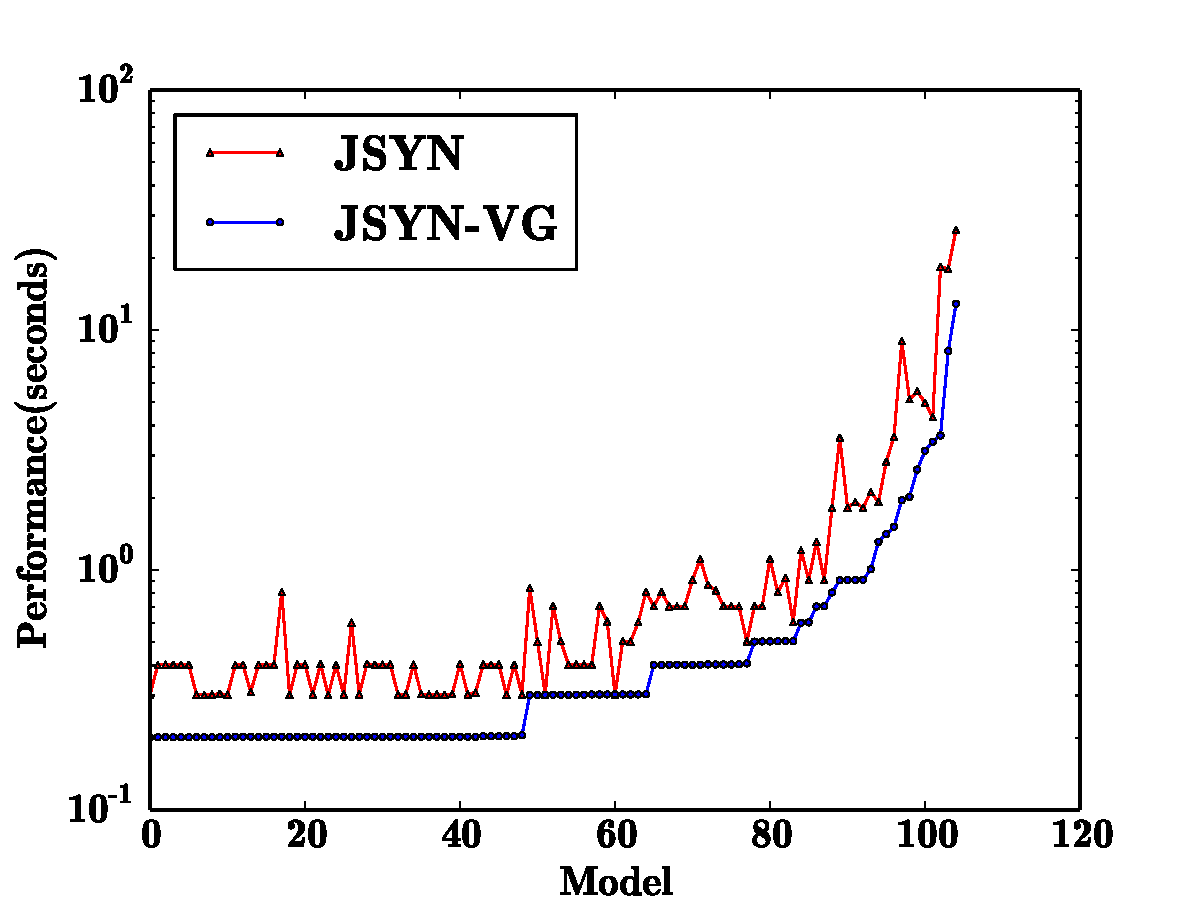
\includegraphics[width=3.5in]{overhead}
\label{fg:performance}}
\hfil
\subfloat[Size of Synthesized
Implementations]{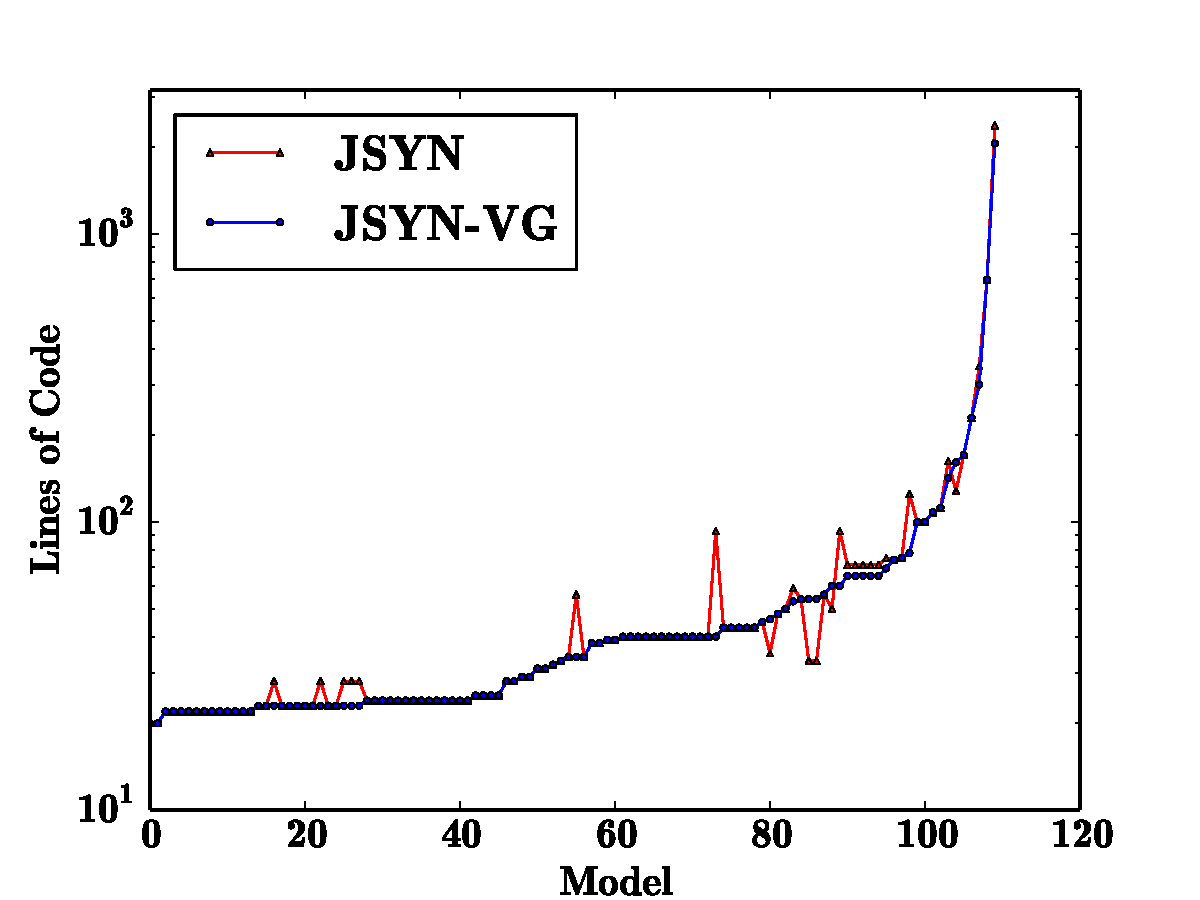
\includegraphics[width=3.5in]{loc}
\label{fg:size}}
\caption{Experimental results}
\label{fg:results}
\end{figure*}


In this section we evaluate \jsynvg by synthesizing implementations
for 115 contracts that originate from a broad variety of contexts. Almost half
of them, 54, come from a collection of contracts that were initally used for
the verification of existing handwritten implementations. The second
biggest collection in our suite contains 52 contracts that correspond to various
development projects, such as a Quad-Redundant Flight Control System, a Generic
Patient Controlled Analgesia infusion pump, as well as a collection of contracts
for a Microwave model, written by graduate students as part of a software
engineering class. The remaining nine models contain variations of the
Cinderella-Stepmother game and the example in Section~\ref{sec:pre}.

Since \jkind already supports synthesis through \jsyn, we were able to directly
compare \jsynvg against \jsyn's k-inductive approach.
The comparison spans over multiple factors, including
algorithm performance, number of problems solved and, finally, performance
of C implementations through the translation of witnesses using \smtlibtoc. We
ran the experiments using a computer with Intel Core i3-4010U 1.70GHz CPU and
16GB RAM.

\begin{table}[!t]
\centering
\caption{Benchmark Statistics}
\label{tbl:stats}
\begin{tabular}{@{}lll@{}}
\toprule
 & \jsyn & \jsynvg \\ \midrule
Problems solved & 110 & \textbf{115} \\
Performance (avg - seconds) & 2.71 & \textbf{1.24} \\
Performance (max - seconds) & 159.05 & \textbf{64.89} \\
Implementation Size (avg - Lines of Code) & 74.45 & \textbf{69.77} \\
Implementation Size (max - Lines of Code) & 2382 & \textbf{2062} \\
Implementation Performance (avg - ms) & \textbf{56.57} & 58.47 \\
Implementation Performance (max - ms) & \textbf{464.359} & 485.197 \\
\bottomrule
\end{tabular}
\end{table}

A listing of the statistics that we tracked while running experiments is
presented in Table~\ref{tbl:stats}.
Figure~\ref{fg:performance} shows the time allocated by \jsyn and \jsynvg to solve each problem, with \jsynvg
outperforming \jsyn across the board, often times by a margin greater than
50\%. Figure~\ref{fg:size} on the other hand, depicts small differences in the
overall size between the synthesized implementations. While it would be
reasonable to conclude that there are no noticable improvements, the bigger
picture is different. The key factor that is not apparent from this figure, is the length of the k-inductive proof. For the majority of the benchmarks in the suite, \jsyn proves their realizability by constructing proofs of length $k=0$, which essentially means
that the entire space of states is an inductive invariant. As such, \jsynvg
also manages to synthesize implementations without requiring any refinement
process. For these cases, both algorithms generate a single Skolem function. In the general case though, the size of \jsyn solutions is directly
dependent on $k$, since each implementation is composed of $k$ Skolem
functions ($k-1$ to initialize the system, and one last for the inductive step),
where the equivalent solution from \jsynvg is always just one.
Figure~\ref{fg:size} hints towards this intuition, through a handful of spikes
in \jsyn implementation size. Despite this, we also noticed cases where \jsyn
implementations are shorter. This provides us with another interesting
observation regarding the formulation of the problem for $k=0$ proofs. In
these cases, \jsyn proves the existence of viable states, starting from a set
of \textit{pre-initial} states, where the contract does not need to hold. This
has direct implications to the way that the $\forall\exists$-formulas are
constructed in \jsyn's underlying machinery, where the assumptions are ``baked''
into the transition relation, affecting thus the creation of Model-Based
Projections by \aeval.



\begin{figure}[h]
\centering
 \begin{Verbatim}[fontsize=\scriptsize]
 ++++++++++++++++++++++++++++++++++++++++++++++++++++++++++
      UNREALIZABLE || K = 6 || Time = 2.017s
                 Step
      variable      0    1      2      3      4      5
      INPUTS
      i1            0    0      0 0.416* 0.944* 0.666*
      i2            1    0 0.083* 0.083*      0 0.055*
      i3            0    1 0.305*    0.5 0.027* 0.194*
      i4            0    0 0.611*      0      0 0.027*
      i5            0    0      0      0 0.027* 0.055*
 
      OUTPUTS
      e             1    3      1      5      4      5
 
      NODE OUTPUTS
      guarantee   true true   true   true   true  false
 
      NODE LOCALS
      b1            0    0      0 0.416* 1.361* 0.666*
      b2            0    0 0.083* 0.166* 0.166* 0.222*
      b3            0    1 1.305* 1.805* 1.833* 2.027*
      b4            0    0 0.611* 0.611*      0 0.027*
      b5            0    0      0      0 0.027* 0.055*
 +++++++++++++++++++++++++++++++++++++++++++++++++++++++++
 \end{Verbatim}
\caption{Spurious counterexample for Cinderella-Stepmother example using \jsyn}

\label{fg:cex}
\end{figure}

Figures~\ref{fg:performance} and~\ref{fg:size} do not cover the entirety of the
benchmark suite. From the original 115 files, five of them cannot be
solved by \jsyn's k-inductive approach. Four of these files are variations of
the cinderella-stepmother game that we described in Section~\ref{sec:example},
using different representations of the game, as well as two different values
for the bucket capacity (2 and 3). Using the variation that we included in the
aforementioned section as an input to \jsyn, we receive an ``unrealizable'' answer, with the counterexample shown
in Figure~\ref{fg:cex}. Reading through the feedback provided by \jsyn, it is
apparent that the underlying SMT solver is incapable of choosing the correct
buckets to empty, leading eventually to a state where an overflow occurs for the
third bucket. As we already discussed though, a winning strategy exists for the
cinderella, as long as the bucket capacity $c$ is between 1.5 and 3. This
provides an excellent demonstration regarding the inherent weakness of \jsyn
in providing sound ``unrealizable'' results. \jsynvg's validity-guided approach,
on the other hand, was able to prove the realizability for these contracts, as
well as synthesize an implementation for each.

 One last statistic that we tracked was the performance of the synthesized C
 implementations. For this purpose, we translated the
 generated witnesses from \jsyn and \jsynvg solutions using
 \smtlibtoc under the same set of options. Table~\ref{tbl:stats} shows that
 while \jsyn implementations are faster, the difference is insignificant enough
 to prevent concerns. The deciding factor in this context is the
 difference in complexity of the Model-Based Projections that get generated by
 \aeval using \jsyn and \jsynvg, with the latter versions containing richer
 expressions, mainly due to the refinement process.

Overall, \jsynvg's validity-guided approach provides significant advantages
over the k-inductive technique followed in \jsyn, and effectively expands
\jkind's solving capabilities regarding specification realizability. The most
significant contribution, however, is the applicability of this approach, as it
is not tied to a specific environment since it can be extended to support more
theories, as well as categories of specification.
